\PassOptionsToPackage{unicode=true}{hyperref} % options for packages loaded elsewhere
\PassOptionsToPackage{hyphens}{url}
%
\documentclass[]{article}
\usepackage{lmodern}
\usepackage{amssymb,amsmath}
\usepackage{ifxetex,ifluatex}
\usepackage{fixltx2e} % provides \textsubscript
\ifnum 0\ifxetex 1\fi\ifluatex 1\fi=0 % if pdftex
  \usepackage[T1]{fontenc}
  \usepackage[utf8]{inputenc}
  \usepackage{textcomp} % provides euro and other symbols
\else % if luatex or xelatex
  \usepackage{unicode-math}
  \defaultfontfeatures{Ligatures=TeX,Scale=MatchLowercase}
\fi
% use upquote if available, for straight quotes in verbatim environments
\IfFileExists{upquote.sty}{\usepackage{upquote}}{}
% use microtype if available
\IfFileExists{microtype.sty}{%
\usepackage[]{microtype}
\UseMicrotypeSet[protrusion]{basicmath} % disable protrusion for tt fonts
}{}
\IfFileExists{parskip.sty}{%
\usepackage{parskip}
}{% else
\setlength{\parindent}{0pt}
\setlength{\parskip}{6pt plus 2pt minus 1pt}
}
\usepackage{hyperref}
\hypersetup{
            pdftitle={Systematic review and climate change analysis in Los Lagos Region},
            pdfauthor={Derek Corcoran},
            pdfborder={0 0 0},
            breaklinks=true}
\urlstyle{same}  % don't use monospace font for urls
\usepackage[margin=1in]{geometry}
\usepackage{longtable,booktabs}
% Fix footnotes in tables (requires footnote package)
\IfFileExists{footnote.sty}{\usepackage{footnote}\makesavenoteenv{longtable}}{}
\usepackage{graphicx,grffile}
\makeatletter
\def\maxwidth{\ifdim\Gin@nat@width>\linewidth\linewidth\else\Gin@nat@width\fi}
\def\maxheight{\ifdim\Gin@nat@height>\textheight\textheight\else\Gin@nat@height\fi}
\makeatother
% Scale images if necessary, so that they will not overflow the page
% margins by default, and it is still possible to overwrite the defaults
% using explicit options in \includegraphics[width, height, ...]{}
\setkeys{Gin}{width=\maxwidth,height=\maxheight,keepaspectratio}
\setlength{\emergencystretch}{3em}  % prevent overfull lines
\providecommand{\tightlist}{%
  \setlength{\itemsep}{0pt}\setlength{\parskip}{0pt}}
\setcounter{secnumdepth}{5}
% Redefines (sub)paragraphs to behave more like sections
\ifx\paragraph\undefined\else
\let\oldparagraph\paragraph
\renewcommand{\paragraph}[1]{\oldparagraph{#1}\mbox{}}
\fi
\ifx\subparagraph\undefined\else
\let\oldsubparagraph\subparagraph
\renewcommand{\subparagraph}[1]{\oldsubparagraph{#1}\mbox{}}
\fi

% set default figure placement to htbp
\makeatletter
\def\fps@figure{htbp}
\makeatother

\usepackage[round]{natbib}
\usepackage{booktabs}
\usepackage{longtable}
\usepackage{array}
\usepackage{multirow}
\usepackage{wrapfig}
\usepackage{float}
\usepackage{colortbl}
\usepackage{pdflscape}
\usepackage{tabu}
\usepackage{threeparttable}
\usepackage{threeparttablex}
\usepackage[normalem]{ulem}
\usepackage{makecell}
\usepackage{xcolor}
\usepackage[]{natbib}
\bibliographystyle{plainnat}

\title{Systematic review and climate change analysis in Los Lagos Region}
\author{Derek Corcoran}
\date{2020-11-30}

\begin{document}
\maketitle

{
\setcounter{tocdepth}{2}
\tableofcontents
}
\hypertarget{systematic-review}{%
\section{Systematic review}\label{systematic-review}}

\hypertarget{introduction}{%
\subsection{Introduction}\label{introduction}}

One of the strategic targets of the Convention of Biological Conservation is ``By 2020, at least 17\% of terrestrial and inland water, and 10\% of coastal and marine areas, especially areas of particular importance for biodiversity and ecosystem services, are conserved through effectively and equitably managed, ecologically representative and well connected systems of protected areas\ldots{}''
This emphasizes not only that protected areas (PA) are one of the most effective elements to prevent extinctions hence conserve biological diversity, also future of biological and landscape conservation need planned increment in the number of PA and effectiveness in terms of strategic allocation of management and economic efforts \citep{le2013protected, watson2014performance}.
This is why the last decades aspects such as economic limitations and the impact on local stakeholders are been taking into account in order to declare news PA and not only its selection based in ecological knowledge \citep{borrini2004indigenous}.

South America has one of the highest proportions of pa area in the world (15.9\%, \citet{ProtectedAreas}).
In Chile, there are 211 PA in its extension. From those, 187 have national jurisdiction and only 24 international.
In southern Chile, Los Lagos Region is named given this region has the largest proportion of lake's area in the country, with 52 lakes over 3 \(Km^2\), and a total area of 2,850 \(Km^2\). It has a population of 828,708 \citep{Censo2017} and an extension of 48,583.60 \(Km^2\).
This region bases its economy in activities related to primary sectors: livestock, aquaculture and forestry industry \citep{BNC_LosLagos}. Even more, Los Lagos Region presents one of the biggest growth in fisheries and aquaculture growth in comparison with the rest of the country during the last 30 years \citep{Soto-alvaradoDesarrollo}.

According to \citet{ProtectedAreas}, Los Lagos Region has 21 PA with 15,777 \(Km^2\) of surface.
An even when includes a large part of the territory, there has been a disconnection with local communities.
This could be because from those 21 PA in the Region, 9 correspond to National Parks (NP) and Natural Monuments (NM) which are IUCN categories that reinforce strict conservation \citep{dudley2008guidelines}.
In addition to that, remoteness of PA can generate disconnection. Given most of the PA are located in remote places, people from developed urban centers do not have, in most of the cases, nexus with those PA and their territory \citep{joppa2009high}
Another factor could be a social phenomena, where cultural changes generate a sense of not sharing a common notion of territory (Montecinos, 2009, p.~24). In the region, this could be a product of economic activities such as salmon farming, where the dependency on international markets predominates.

Among the PA in Los Lagos Region, there are three Andean National Parks: Puyehue National Park (PNP), Vicente Perez Rozales National Park (VPRNP), and Alerce Andino National Park (AANP). PNP, VPRNP, and AANP as all national PA in Chile are under the supervision and administration of the National Forestry Corporation (CONAF). They count with management plans (2008, 2015, and 1997, respectively), which provide a very careful compilation of data. However, these documents have not been correctly updated and they have a lack of information with the changes that have occurred in the last years. For example, between 1995 and 2016 native forests in this area have suffered important losses because of land use changes (mostly land modification to grassland and shrubs).
Hence, the area presents an increment of vulnerability in front of climate change \citep{marquet2019biodiversidad}.

Considering relations of PA and local communities, and the importance of the expansion of ecological knowledge to areas that resume the complexity of each PA in order to face specific perturbations or global problematic as climate change in the future, should be a fundamental step in Chile to assure a correct management and projection of PA to the future.
This review revise the ecological literature carry out in these three protected areas and its surroundings in Los Lagos Region in order to generate a base line that allow to project scenarios of climate change to systematic conservation planning in PA.
We made a systematic review of research searching by the names of the three PA: PNP, VPRNP, and AANP; and by the geographical area of Southern Chile.
Doing so, we were able to identified tendencies and gaps in research developed in these three National Parks. We could defined a vision on where to focus new studies that allow systematic conservation plans that includes information to deal with climate change and ensure the biological diversity in Southern Chile.

\hypertarget{methodology}{%
\subsection{Methodology}\label{methodology}}

In order to identify research developed in the focus area, a systematic review of literature was performed through the Web of Knowledge database. Information was categorized according to research areas presented in this project.
Two eligibility criteria were performed: 1. including the name of the National Parks of interest, using keywords at topic level: ``Puyehue National Park'' or ``Vicente Perez Rozales National Park'' or ``Alerce Andino National Park'', and 2. Geographic areas surrounding the National Parks, using keywords at topic level: ``South Central Chile'' or ``North Chilean Patagonia'' or ``Los Lagos Region''. The period of the search included from 1975 until October 2020. Grey-literature was not incorporated in the selection.

Articles selected were categorized by publication year, source title, keywords used, and categories created for the purpose of this review: key component, study location, methodology used, process involved, and study object.
Key components categorized articles according to area of study. This classification included Archaeology \& Paleoecology, Climate \& environment (including studies in climate, environmental conditions, and seismology), Ecosystem functioning \& services, Freshwater biodiversity, Hydrology, Social-ecology, and Species \& distribution (including biogeography, species description, and exotic species).

Study location encompassed categories such as the three National Parks of interest: AANP, PNP, and VPRNP; adjacent areas to NP: Adjacent to AANP, Adjacent to PNP, Adjacent to VPRNP; similar ecosystems to NP: Andes of Los Rios Region, Argentinian Andes, and Neuquen in Argentina; Larger areas that comprise NP: Los Lagos Region, 2 regions, 3 regions, 4 regions, 5 regions, More than 5 regions; Global studies: Chile, Chile \& Argentina; and Close urban centers: Valdivia.

Methodology classified articles based in how data was collected and/or analysed.
Methods included data from the field: field survey, field collection (similar a survey but with samples that need further processes to be analysed, such as dendrochronology or electric fishing), field experiment (that requires modification to one or more conditions in a location, such as transplant or seedling experiments).
Other classifications were modeling (including data analysis such as simulations, correlational and multivariate models, and spatial models), molecular analysis (reconstruction of mt-DNA, isotopes, and genetic analysis), and reviews of literature.
There is a category of social methods, that include both quantitative (surveys an questionnaires) and qualitative (interviews and discussion articles).
Process category makes reference to the question behind the articles and implies which is the mechanism studied (see the list of of 47 options in Table \ref{tab:tabProcess}).

\begin{table}

\caption{\label{tab:tabProcess}Processes mentioned in studies}
\centering
\begin{tabular}[t]{l}
\toprule
Process\\
\midrule
Behavior\\
Chemical composition\\
Climate\\
Climate change\\
Collective action\\
\addlinespace
Communication\\
Community ensemble\\
Composition\\
Connectivity\\
Conservation\\
\addlinespace
Decomposition\\
Distribution\\
Epidemiological\\
Erosion\\
Eutrophication\\
\addlinespace
Feeding\\
Fire activity\\
Fixation\\
Flow prediction\\
Flowering\\
\addlinespace
Forest characterization\\
Functional variation\\
Genetic variability\\
Genetic variation\\
Growth\\
\addlinespace
Iconography\\
Infiltration\\
Invasion\\
LULC\\
Parasitation\\
\addlinespace
Participation\\
Past climate change\\
Past distribution\\
Phylogeography\\
Political-ecology\\
\addlinespace
Pollution\\
Productivity\\
Rainfall partitioning\\
Regeneration\\
Runoff\\
\addlinespace
Seasonal variability\\
Sedimentation\\
Social vulnerability\\
Succession\\
Survival\\
\addlinespace
Topography\\
Vulnerability\\
\bottomrule
\end{tabular}
\end{table}

Study object classification was prepared based on what is the minimum element studied in each article. This included living organisms such as humans (household combustion, people, and urban areas), animals (communities of birds, crustacean, fishes, and herpetofauna; species of Aegorhinus, craspedacusta, Dromiciops, Liolaemus, wild boar, and woodwasp), plants (aquatic plants, Chusquea, Embothrium, ferns, native vegetation, pollen, Proteaceae, Sarmienta), other organisms (such as cyanobacteria, Didymosphenia, lichens, and protozoa), and a particular living category given its abundance of publications is forest communities (with focus in one species Austrocedrus, \emph{F. cupressoides}, and Nothofagus; or in more diverse environments as coihue-Rauli-Tepa, forest, native forest, and evergreen trees).

Study objects also included non-living organisms, focusing in geographic elements (basins, groundwater Storage, lakes, runoff, streams, watershed, and also soil and regional subdivision), physical conditions (fires, precipitation, particulate matter, rock art), and data bases.

In order to centered this review in ecological knowledge carry out in the area of study, we focus our search in Los Lagos region research and Andean studies in surrounded areas. We left out coastal systems within the region, specially research based on Chiloé island because local communities keep a traditional way of life and agricultural systems. This was even proposed as Global Importance Agricultural Heritage System (GIAHS) by the Food and Agricultural Organization \citep{FAO2003Chiloe, FAO2008Chiloe}.

\hypertarget{results}{%
\subsection{Results}\label{results}}

There is a large amount of research related to Southern Chile. Isi Web of Knowledge database identified 874 records that fitted keywords, of those 520 articles were screened, and 441 full-text articles were assessed for eligibility.

A total of 121 articles were selected in this review. From those 17 articles were find from the three National Parks and 104 articles from searching nearby areas of them.

\begin{figure}
\centering
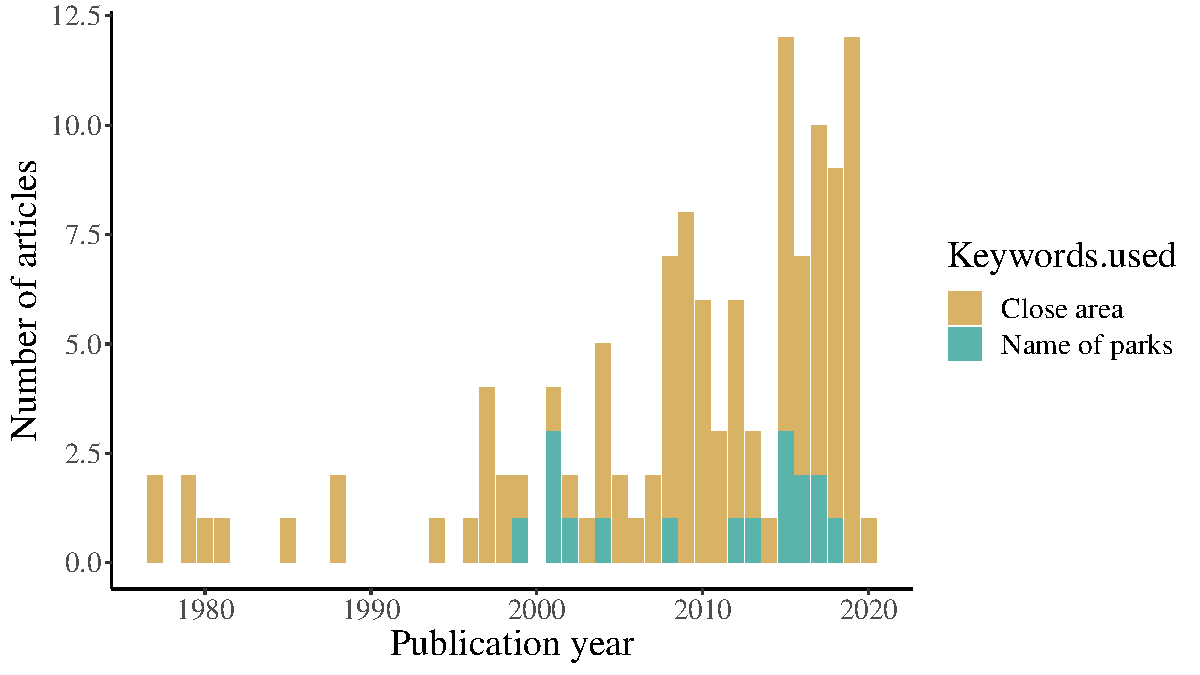
\includegraphics{Review_and_climate_files/figure-latex/Years-1.pdf}
\caption{\label{fig:Years}Temporal distribution of articles according to keywords used in this review of literature}
\end{figure}

In general terms, number of articles have been increasing during the years. However there are a few years, such as 2003, 2006, 2014, and 2020 that show a striking decrease in publications (Fig \ref{fig:Years}). Studies in NP do not show a pattern during the years, only two picks in publications: in 2001 and 2015.

\begin{figure}
\centering
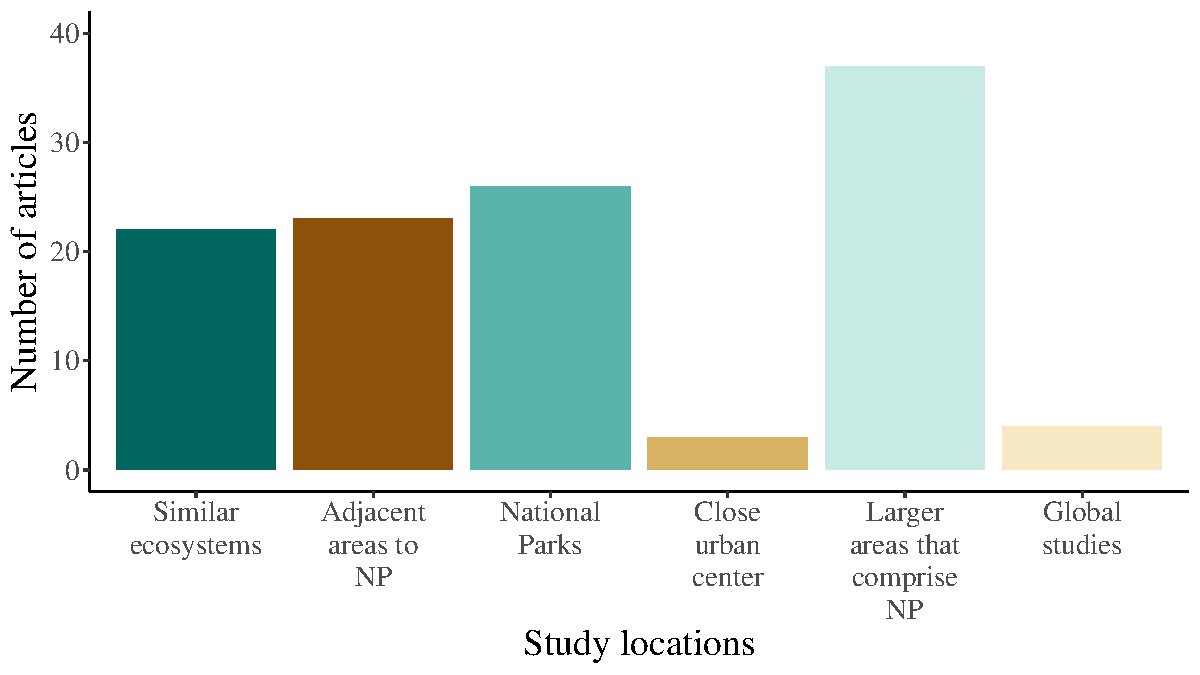
\includegraphics{Review_and_climate_files/figure-latex/Locations-1.pdf}
\caption{\label{fig:Locations}Locations where studies were carry out}
\end{figure}

From the articles carry out in the NP of interest, only 20 articles were carry out in PNP, 4 in AAPN and 2 in VPRPN.
Adjacent areas to these three NP comprehended 23 studies. Similar ecosystems, as those found in Andes of Los Ríos Region and Neuquén Province in Argentina, also showed high number of publications 22. However, most of the articles (37) studied larger areas that comprises Los Lagos Region and the three NP (Fig \ref{fig:Locations}).

\begin{figure}
\centering
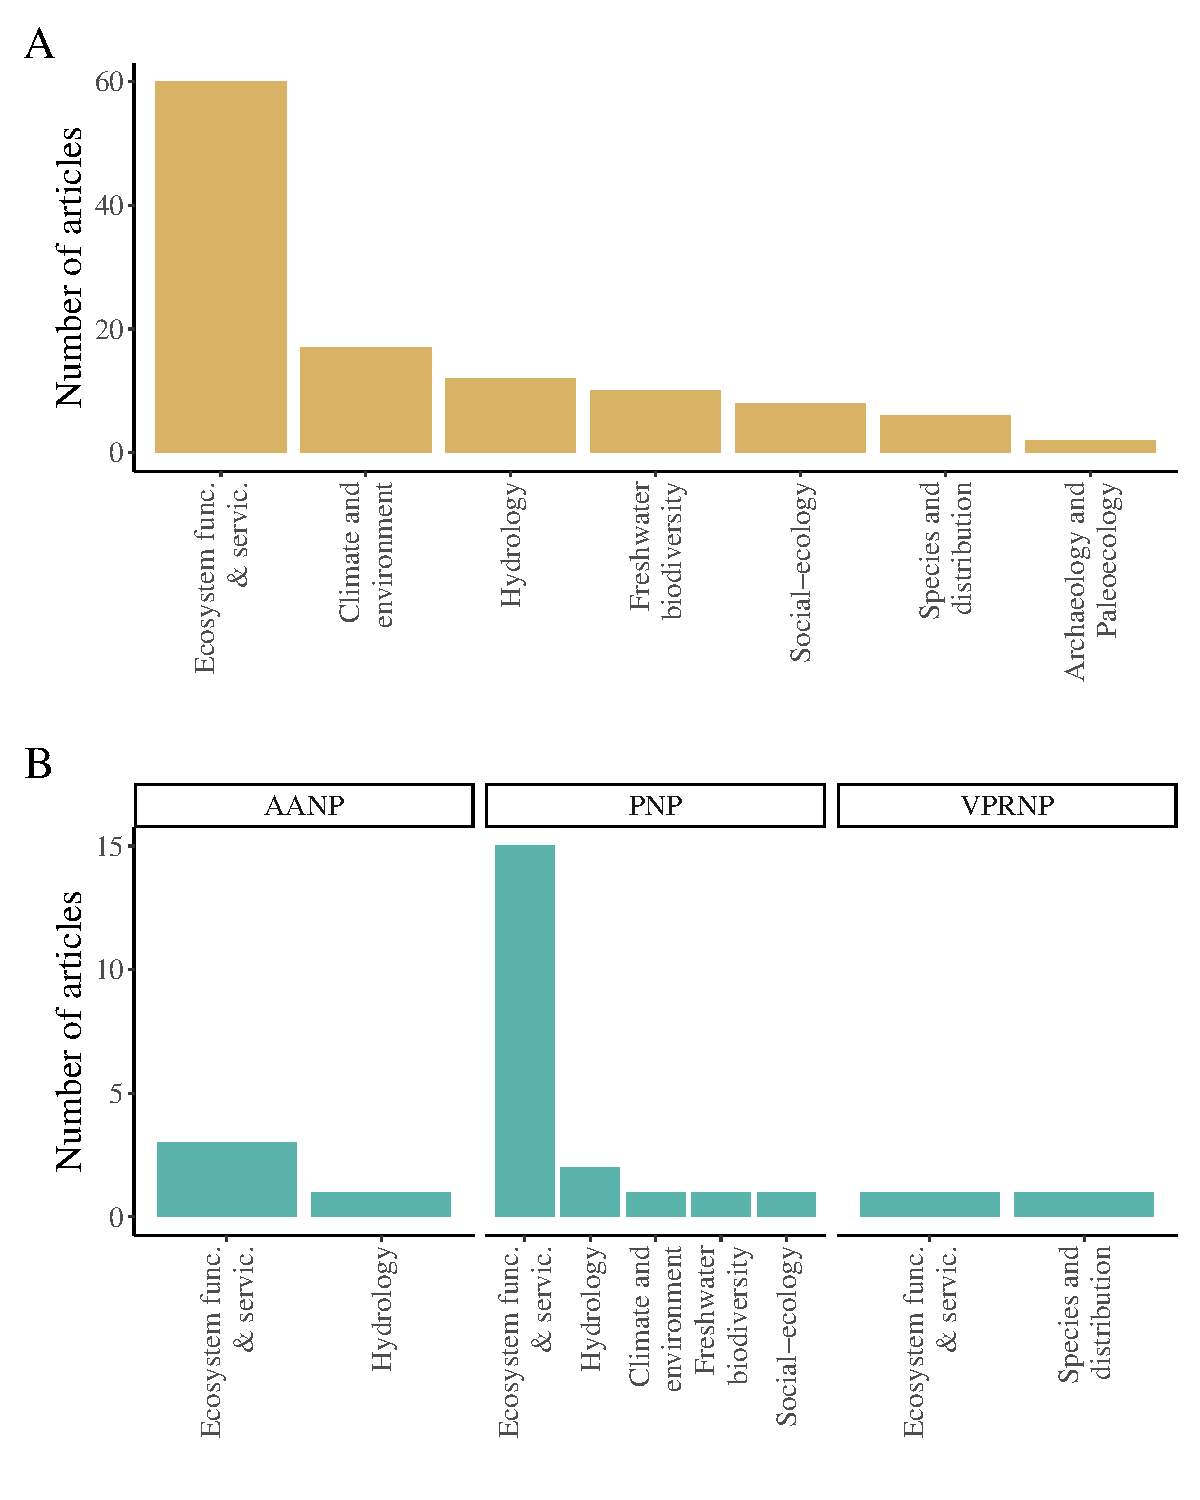
\includegraphics{Review_and_climate_files/figure-latex/Areas-1.pdf}
\caption{\label{fig:Areas}Areas of study. A, study areas for all articles. B, study areas for articles focused in the three NP.}
\end{figure}

According to study areas, half of the studies are focus on ecosystem functioning and services (49.59\%). The rest of the studies does not exceed the 20 articles each. They are in decreasing number: Climate and environment, Hydrology, and freshwater biodiversity studies. The rest of the areas have less than 10 articles published (Fig \ref{fig:Areas}).
In addition, Ecosystem functioning and services has been studied in the three NP, however its proportion in PNP is notably higher than the other NP. Additionally, PNP is the only NP that shows several areas of study, even with only a few articles. In terms of area of study, Hydrology is the next area with more studies in NP with mention in AANP and PNP.

\begin{figure}
\centering
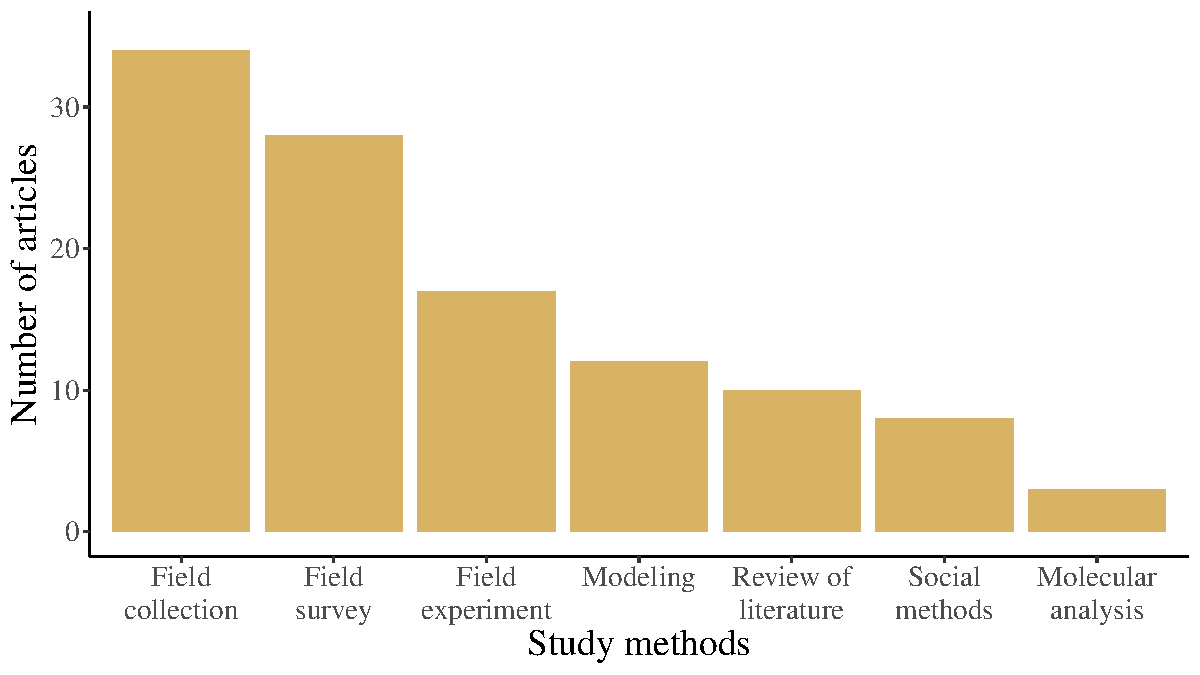
\includegraphics{Review_and_climate_files/figure-latex/Methods-1.pdf}
\caption{\label{fig:Methods}Methods used in selected articles of this review.}
\end{figure}

Data collected from the field is abundant and represents a 65.29 \% of the studies. Among field collection, it highlights some studies where there is some specific collection of data through methods such as dendrochronology (5 articles) or electric fishing (2), (Fig \ref{fig:Methods}).
Modeling category included 12 articles taking into account correlational, multivariate , and spatially explicit models.
Review of literature was mention in 10 articles and social methods that encompasses communicational strategies, discussion articles, both quantitative and qualitative methods, surveys, and interviews comprehended only in 8.
The least used method in this review is molecular analysis (only 3), and included isotopes, genetic analysis, and reconstruction of mt-DNA.

\begin{figure}
\centering
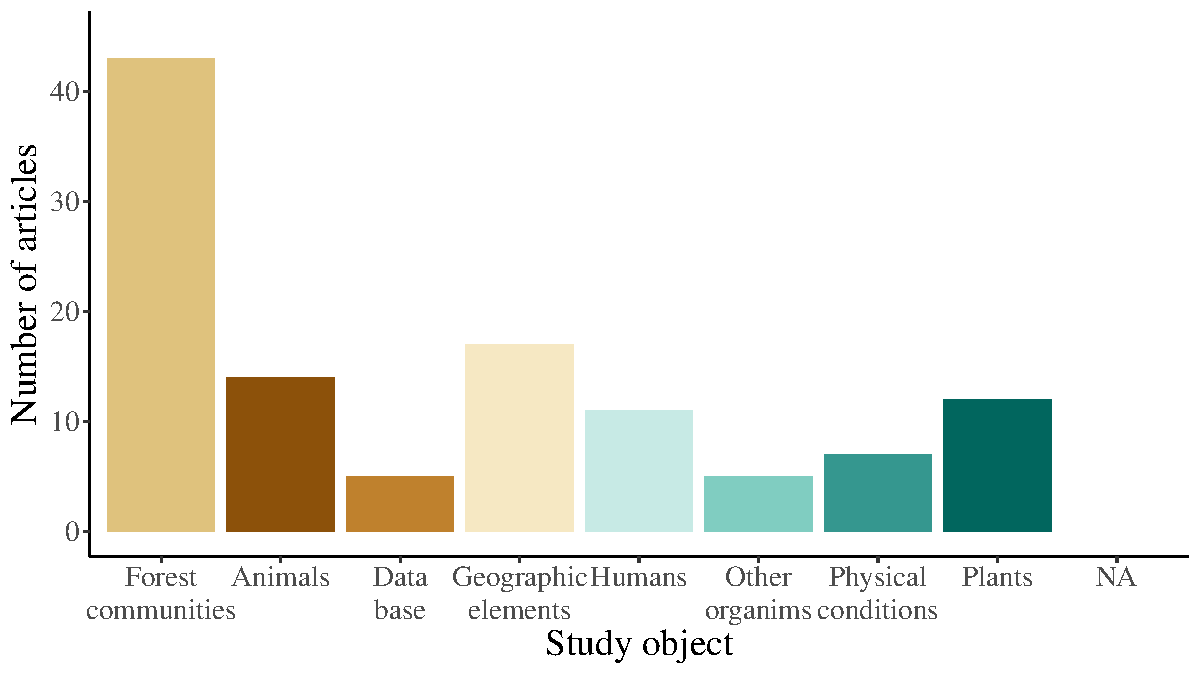
\includegraphics{Review_and_climate_files/figure-latex/Objects-1.pdf}
\caption{\label{fig:Objects}Objects studied in selected articles of this review.}
\end{figure}

Living elements from nature are the most frequent object of study in this review (57.02 \%) (Fig \ref{fig:Objects}). From those, most of the studies are centered in forest communities (43 articles), where articles that studies Nothofagus (20) and Native forest (15) are the majority (Table \ref{tab:GeneralObject}).

\begin{table}

\caption{\label{tab:GeneralObject}Study objects in detail}
\centering
\begin{tabular}[t]{lll}
\toprule
General object & Study object & No of articles\\
\midrule
 & Aegorhinus & 1\\

 & Bird species & 1\\

 & Craspedacusta & 1\\

 & Crustacean & 1\\

 & Dromiciops & 2\\

 & Fishes & 3\\

 & Herpetofauna & 1\\

 & Liolaemus & 1\\

 & Salmonids & 1\\

 & Wild boar & 1\\

\multirow{-11}{*}{\raggedright\arraybackslash Animals} & Woodwasp & 1\\
\cmidrule{1-3}
 & Database records & 1\\

 & Fire database & 1\\

 & Spatial proyection & 1\\

\multirow{-4}{*}{\raggedright\arraybackslash Data bases} & Temperature records & 2\\
\cmidrule{1-3}
 & Austrocedrus & 1\\

 & Coihue-Rauli-Tepa forest & 1\\

 & Evergreen trees & 3\\

 & F. cupressoides & 2\\

 & Forest & 2\\

 & Native forest & 15\\

\multirow{-7}{*}{\raggedright\arraybackslash Forest communities} & Nothofagus & 20\\
\cmidrule{1-3}
 & Basins & 1\\

 & Groundwater Storage & 1\\

 & Lakes & 8\\

 & Regional subdivision & 1\\

 & runoff & 1\\

 & Soil & 2\\

 & Streams & 1\\

\multirow{-8}{*}{\raggedright\arraybackslash Geographic elements} & watershed & 2\\
\cmidrule{1-3}
 & Household combution & 1\\

 & People & 9\\

\multirow{-3}{*}{\raggedright\arraybackslash Humans} & Urban areas & 1\\
\cmidrule{1-3}
 & Cyanobacteria & 1\\

 & Didymosphenia & 1\\

 & Lichen & 1\\

\multirow{-4}{*}{\raggedright\arraybackslash Other organims} & Protozoa & 2\\
\cmidrule{1-3}
 & Fires & 1\\

 & Particulate matter & 1\\

 & Precipitation & 4\\

\multirow{-4}{*}{\raggedright\arraybackslash Physical conditions} & Rock art & 1\\
\cmidrule{1-3}
 & Aquatic plants & 1\\

 & Chusquea & 4\\

 & Embothrium & 1\\

 & Ferns & 1\\

 & Native vegetation & 2\\

 & Pollen & 1\\

 & Proteaceae & 1\\

\multirow{-8}{*}{\raggedright\arraybackslash Plants} & Sarmienta & 1\\
\bottomrule
\end{tabular}
\end{table}

Studies in species and communities are mention in three groups: 1. Animals with a 11.57\% of the articles, 2. Plants with a 9.92\% and 3. Other organisms with a 11.57\%

Human elements studied only represent 9.09\% of the total of research. This included studies in people (9) and specific interests such as household combustion, and urban areas (only 2 articles)

Geographic objects of study are centered in hydrological elements such as basins, watershed, basins, groundwater storage, runoff, and streams (14 of 16 articles), most of them studied lakes (8 articles).
Physical conditions reunited study objects in a variety from environmental conditions such as precipitation and fire, passing through particular matter and rock art.

\hypertarget{key-components}{%
\subsubsection{Key components}\label{key-components}}

\hypertarget{hydrology}{%
\paragraph{Hydrology}\label{hydrology}}

\begin{figure}
\centering
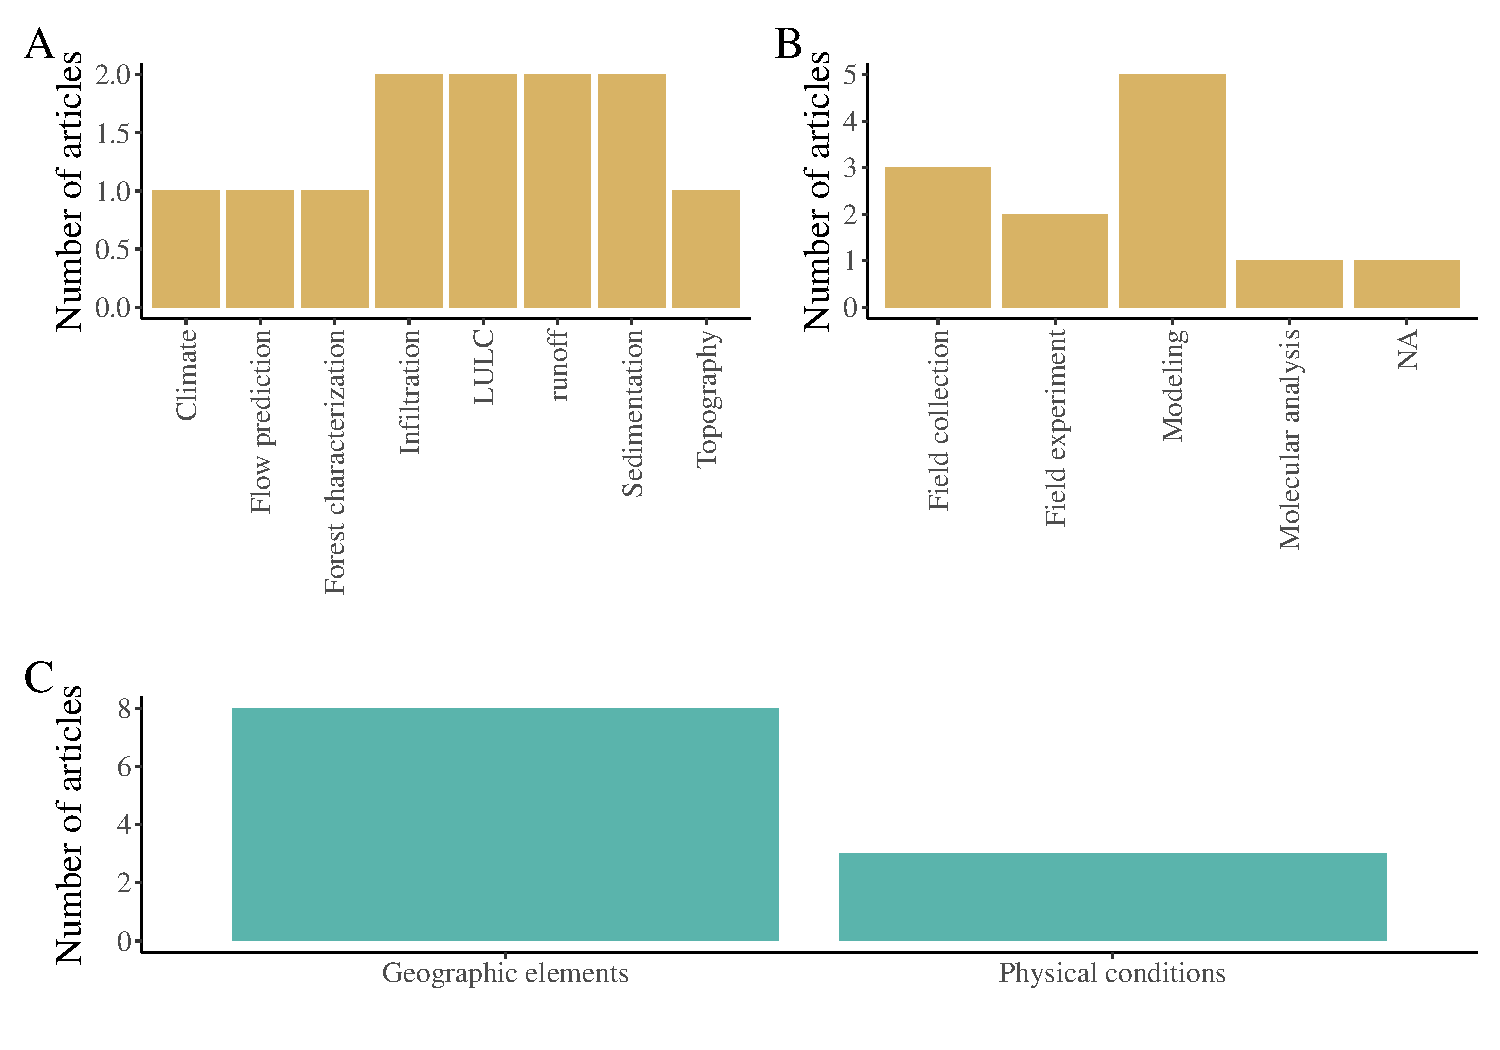
\includegraphics{Review_and_climate_files/figure-latex/Hydrology-1.pdf}
\caption{\label{fig:Hydrology}Articles classified as Hydrological studies. A, study areas. B, Methodologies applied. C, study objects.}
\end{figure}

From the total of articles focused on hydrology (Fig \ref{fig:Hydrology}), most of the processes studied are related to water flows (flow prediction, infiltration, and runoff with a total of 5 articles) and landscape (forest characterization, LULC and topography with 4 articles).
Data from the field (including both field collection and experiments) reaches 5 articles, same as modeling as a methodological resources.
In terms of objects of study, they are mostly geographic elements (8 articles), where half of them studied lakes and precipitation. Physical conditions where only mentioned in 3 articles, all of them studied precipitations.

\hypertarget{ecosystem-functioning-and-services}{%
\paragraph{Ecosystem functioning and services}\label{ecosystem-functioning-and-services}}

\begin{figure}
\centering
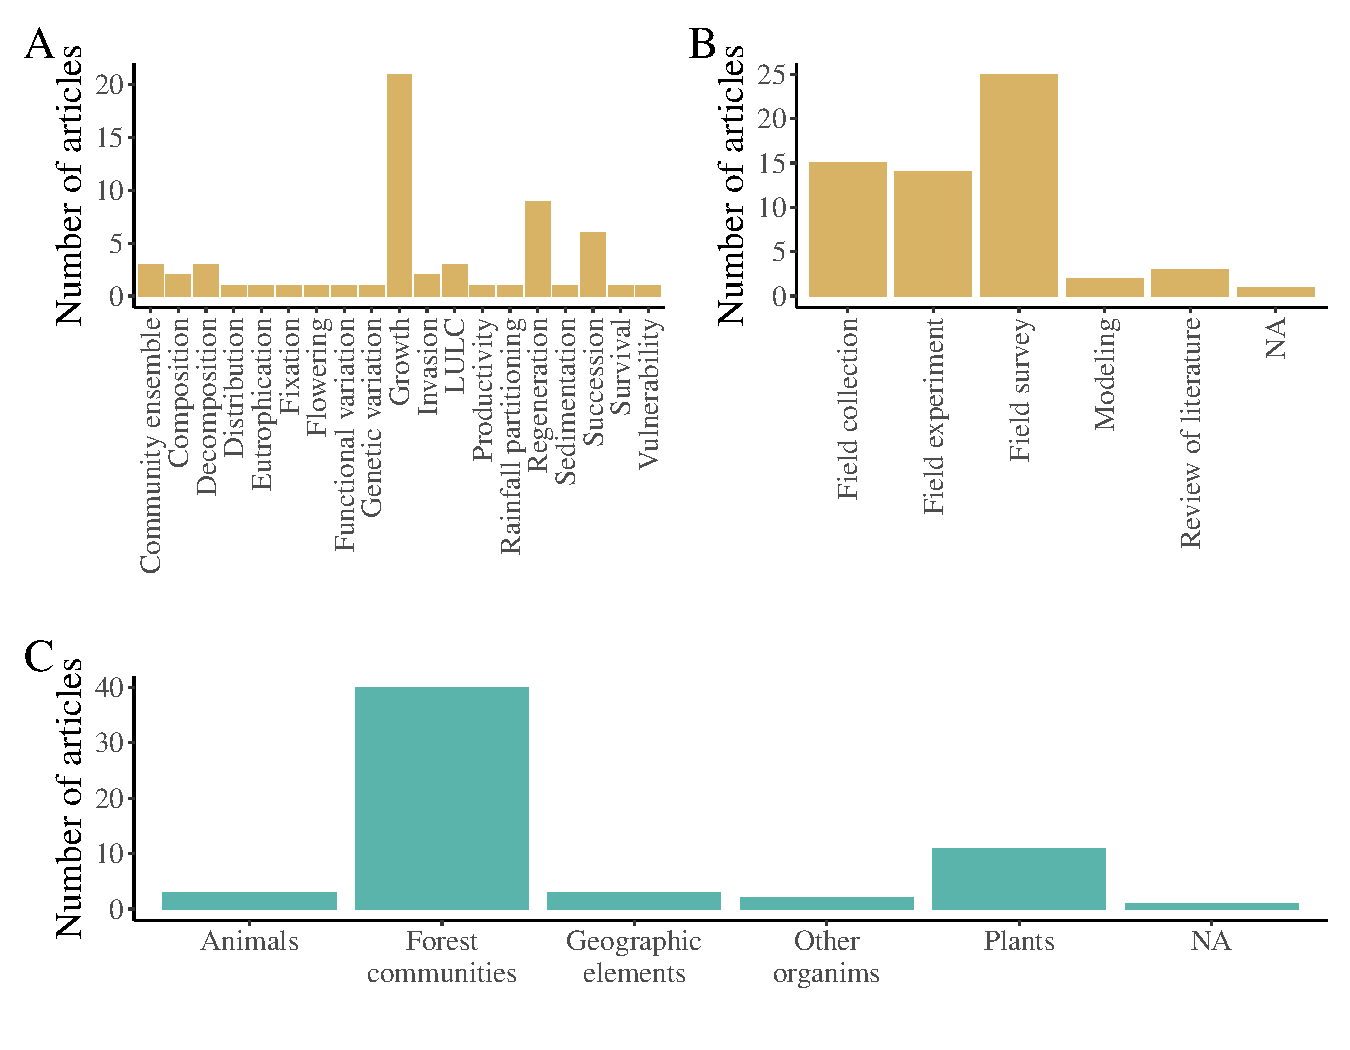
\includegraphics{Review_and_climate_files/figure-latex/Ecosys-1.pdf}
\caption{\label{fig:Ecosys}Articles classified as Ecosystem functioning and services studies. A, study areas. B, Methodologies applied. C, study objects.}
\end{figure}

Ecosystem functioning and services are very diverse in processes studied and aspects related to growth (21 articles), regeneration (9 articles), and succession (6 articles) were the most frequent to find. In terms of methods used, most of the data comes from the field (90\%), being the field survey the most adopted by researchers (25 articles), second field collection with 15 articles and third field experiment with 14 articles.
Study objects in this area are mostly related to forest communities (40 articles). From those, it highlights Nothofagus forests and native forest (20 and 15 articles, respectively).

\hypertarget{freshwater-biodiversity}{%
\paragraph{Freshwater biodiversity}\label{freshwater-biodiversity}}

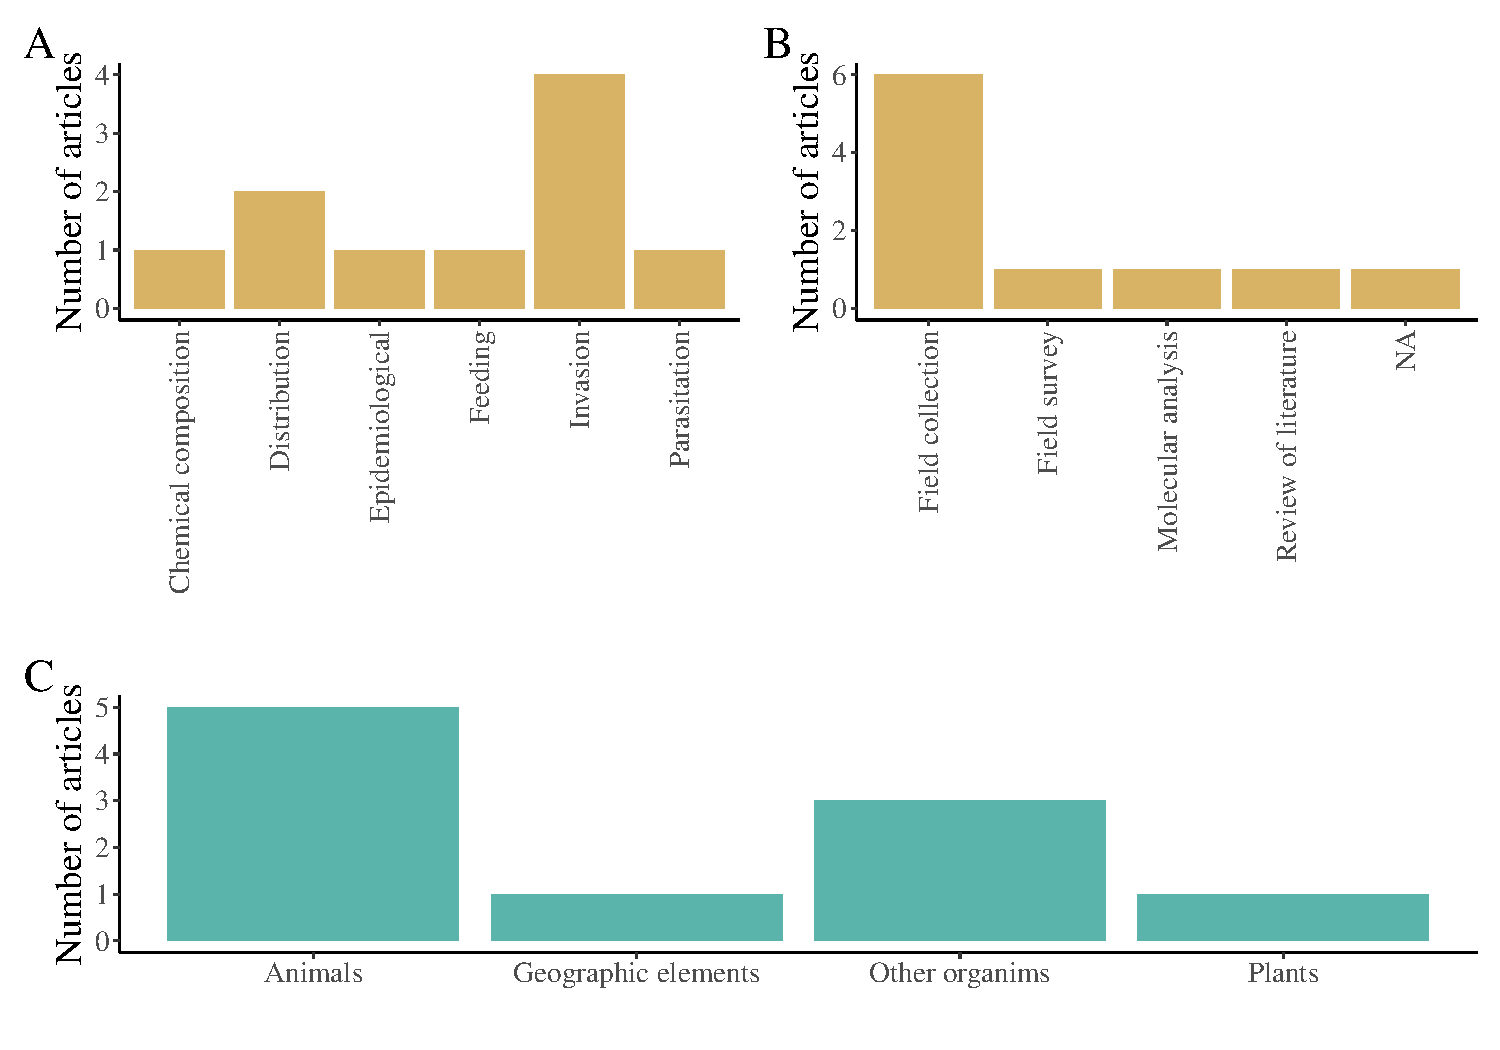
\includegraphics{Review_and_climate_files/figure-latex/Fresh-1.pdf}
Freshwater biodiversity studies focuses mostly in invasion processes (4 articles). Additionally, field collection is the most registered method used (6 articles), this category includes particular activities such as electric fishing and sampling stations.
Object of studies are centered in living organisms with a 90\% of the articles, among them most of the articles studied animals (5 articles, mostly fishes), and other organisms (3 articles, including cyanobacterias, Didymosphenia, and protozoa).

\hypertarget{social-ecological}{%
\paragraph{Social-ecological}\label{social-ecological}}

\begin{figure}
\centering
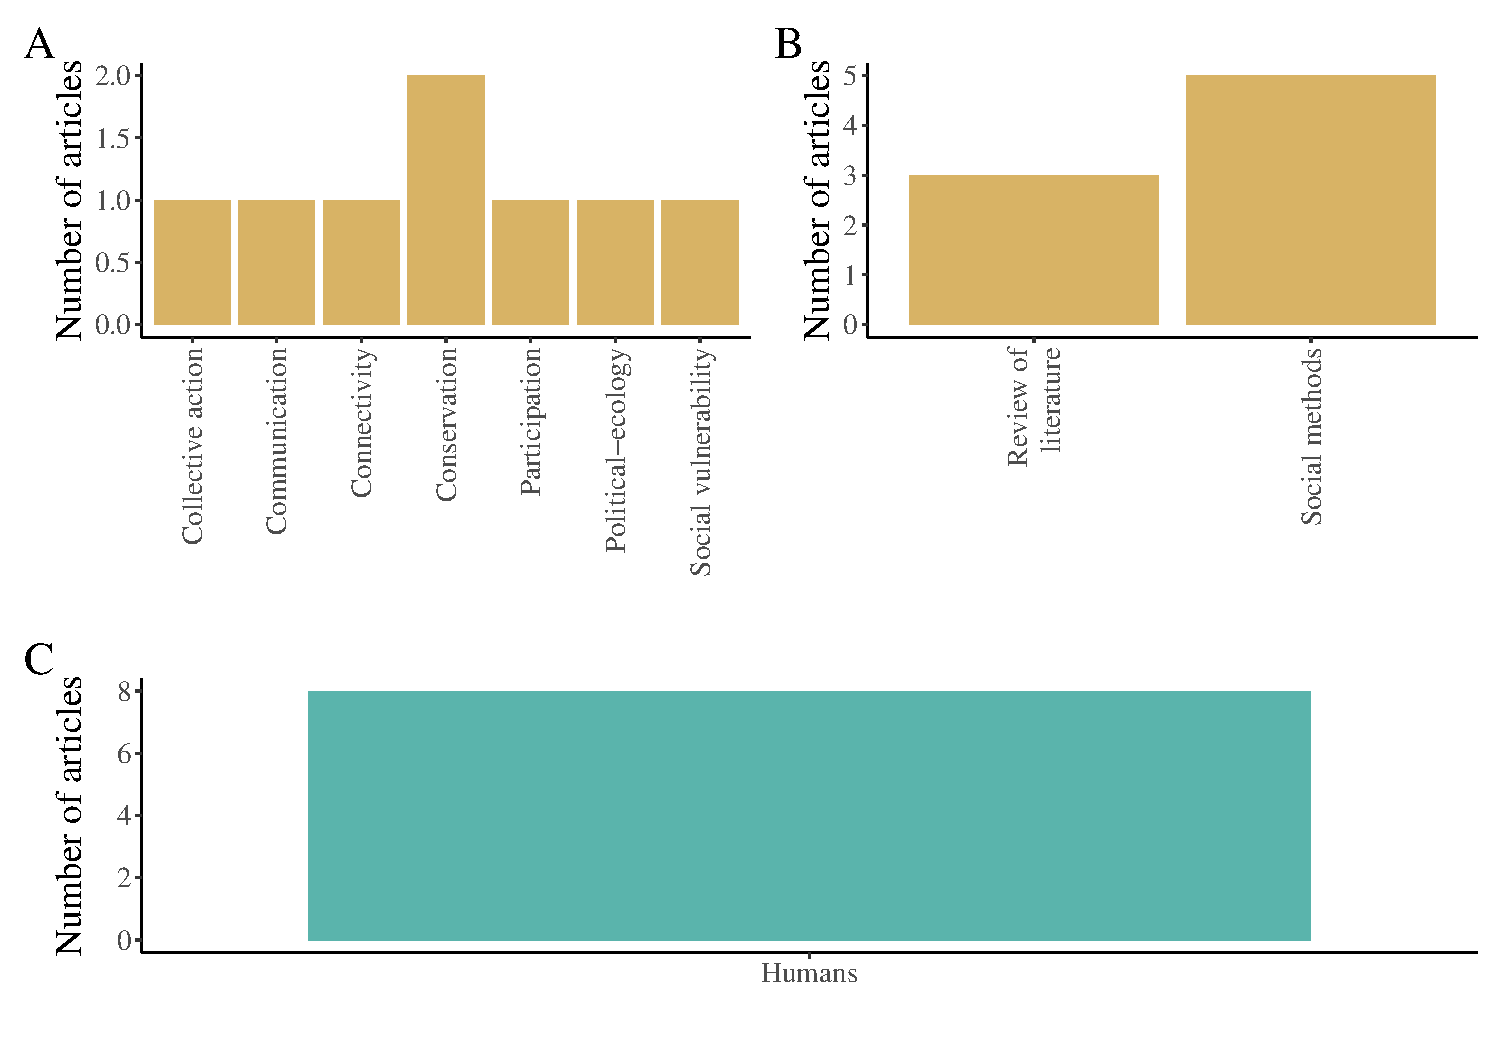
\includegraphics{Review_and_climate_files/figure-latex/Social-1.pdf}
\caption{\label{fig:Social}Articles classified as Social-ecological studies. A, study areas. B, Methodologies applied. C, study objects.}
\end{figure}

Social-ecological research is scarce and processes studied are diverse. However there is a notable environmental concern reflected in aspects as collective action, conservation, participation and political-ecology that involve more than a half of the studies. Methodology involved in this studies are mostly social methods (5 articles), which included quantitative and qualitative such as people's surveys, interviews and articles of discussion based on ethnography, and they are all based in research on people.

\hypertarget{climate-and-environment}{%
\paragraph{Climate and environment}\label{climate-and-environment}}

\begin{figure}
\centering
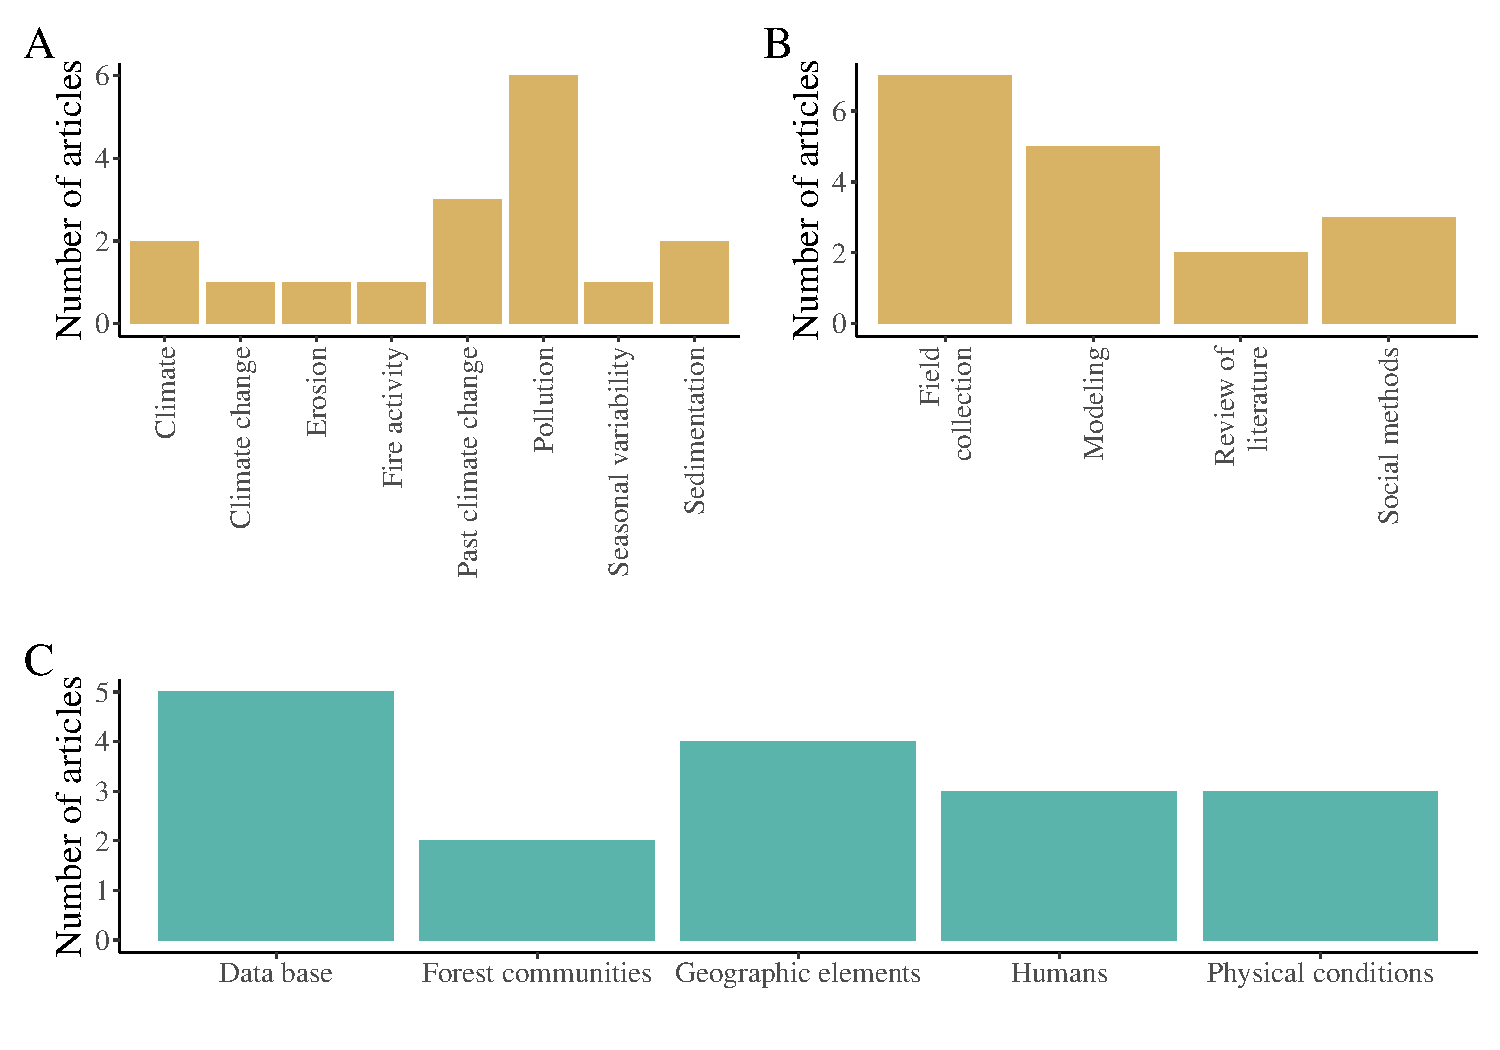
\includegraphics{Review_and_climate_files/figure-latex/Climate-1.pdf}
\caption{\label{fig:Climate}Articles classified as Climate and environment studies. A, study areas. B, Methodologies applied. C, study objects.}
\end{figure}

Climate and environmental area is diverse and showed focus in studies related to pollution with a component of social studies and climate in different scales and times. Among the processes studied, pollution is the most mentioned (6 articles), however the amount of publications centered in climate is not less (current climate 2 articles, climate change 1 article, past climate change 3 articles). Methods used are mostly collections from the field and modeling (41 and 29\%, respectively). Study objects are diverse and involved data bases (5 articles with fire and temperature records or spatial projections), geographic elements (4 articles, including regional subdivision, lakes and soil), humans (3 articles including people and household combustion), physical conditions (3 articles, including precipitation, fires and particulate matter)

\hypertarget{other-key-components}{%
\paragraph{Other key components}\label{other-key-components}}

Species and distribution area focused mostly in distribution of species, phylogeography ans genetic variability (67\% of the articles). More than a half used data from the field and all of the studies found centered in animals. In contrast, archaeology and paleoecology area presented only two articles, one focused in iconography (rock art) and the other centered in past distributions of native forest.

\hypertarget{discussion}{%
\subsection{Discussion}\label{discussion}}

This review provides insight into in ecological studies carry out in three PA: PNP, VPRNP, AANP, and their surrounded geographical areas, that allow to create a baseline of ecological knowledge. Doing so, we were able to identified tendencies and gaps in research developed in these area, in order gather the information needed to generate climate change projections and create systematic conservation plans that ensure the biological diversity in Southern Chile.

The results indicated that most of the studies were focused in ecosystems functioning and services and the other areas of research are poorly studied. There is a gap in social-ecological studies that includes local communities perceptions of NP and their relationship in terms of interactions.
Climate change have been mentioned, but mostly considering aspects of the past and related to local perturbations. This is because the area of study has been continuously modified by natural events such as volcanic activity, with volcanic centers such as Puyehue (2,240 m in PNP), Cordón Caulle (2,236 m; in PNP), Tronador (3,565 m; in VPRNP), Osorno (2,661 m; adjacent to VPRNP) \citep{petit1999cronologia, SternVolcanism}, and earthquakes as Valdivia in 1960 \citep{melnick2018back}.

There is robust research area focused in ecosystem functioning and services. These studies are mostly centered in native forest, where Nothofagus regeneration dynamics is an important point of reference \citep{VEBLEN1979nothofagus, Pollmann2004Nothofagus, Soto2017nothofagus}.
The increment of this studies are important given the development of forestry in southern Chile.
Although high intensive forestry is centered in plantations of exotic species such as Pinus radiata and Eucalyptus, new approaches are considering changes in forestry and landscape management of forest plantations. This includes recovery of native forest patches \citep{salas2016forest} and there is also growing forestry activity applied to natural forests.

Even thought the area of study presents a large number of articles related to forest and its regeneration, there are very few studies related to their threats, particularly on fire activity.
This generate a gap in what is relevant to the area of study because the structure and composition of forest plantations (which are extensive in the area) promotes more fires than native forest of Nothofagus \citep{Gonzalez2018Mega, McWethy2018fire}.
Even thought the area of study presents a large number of articles related to forest and its regeneration, there are very few studies related to their threats, particularly on fire activity.
This generate a gap in what is relevant to the area of study because the structure and composition of forest plantations (which are extensive in the area) promotes more fires than native forest of Nothofagus \citep{Gonzalez2018Mega, McWethy2018fire}. Fire events in similar areas (low access, topography, and climate) have covered large areas and affected native ecosystems. Fires in Torres del Paine National Park in 2012 (17,000 ha), China Muerta National Reserve in 2015 (3,700 ha), and Colonia Sur, Cochrane in 2019 (15,000 ha) were registered as very difficult to control \citep{Arroyo2019COP}.

The regions that were most affected by fires during the MD were Maule, Biobio, and Araucania (35 to 39°S) that concentrate 75\% of forest plantations in Chile. Although both maximum temperatures and precipitation are drivers of fire activity, analysis indicates that the sustained rainfall deficit during 2010 and 2015 was the most critical factor in the enhanced fire activity \citep{Gonzalez2018Mega}.

From the few studies found in social-ecological area, there are some characterizations of local actors and their relation with NP.
\citet{SozaAmigoTurism} studied the movement of people between urban centers and PNP. Here, the authors evaluated the
connection with PNP with three nearby cities: Valdivia, Osorno, and Puerto Montt with 154,716; 147,826 and 220,143 of urban population respectively \citep{Censo2017}.
The results show that the changes in the economic structure had improve the main sectors of urban centers, weakening the potential development of the NP. Especially the lacks of connectivity development and the small supply of good and services of the NP are the main constraint that arise from the analysis to increase the number and length of visits.
A map of local actors developed by \citet{mardones_social} and their network properties showed high fragmentation of social network according to economic sectors (agriculture, artisan fisheries, tourism, among others) and low participation and separation from the PA which has not incorporated the community.
Both studies seems to demonstrate a sentiment described in local sociology, that provinces in this region do not share a common notion of territory or a regional common agenda. This has been explain as cultural change as a product of economic activities such as salmon farming, where the dependency of international markets predominates (Montecinos, 2009, p.24). The lack of participation is also a reflection of a bad distribution of equity, and refers to the fair distribution of benefits of PA \citep{zafra2019progress} and is one of the AICHI targets for PA.

Among freshwater diversity articles, there are contributions with description of species either by studies on invasions \citep{Urrutia2017invasive, Esse2018spectral, Fuentes2019lakes}, distribution of native species \citep{Zapata2008Protozoa, Unmack2009hatcheria} or more specific aspects such as parasitation in fishes \citep{GeorgeNascimento2009} and feeding \citep{Beltran2012dietary}. Among the contributions made by studies in hydrology, there are some characterization of lakes through sedimentation \citetext{\citealp[organic matter preserved in a lake and its watershed:][]{Bertrand2010bulk}; \citealp[environmental impacts associated with increasing industrial activities and land degradation:][]{Fagel2010geochemical}} and infiltration of precipitation \citetext{\citealp[hydrochemical fluxes in a Nothofagus pumilio forest:][]{Godoy1999Hydrochemical}; \citealp[chemical composition of bulk precipitation:][]{Godoy2001precip}}, with the last two studies carry out in PNP. There are some more research regarding hydrology, however they describe processes close to the coast of Los Lagos and Los Rios Regions in the valdivian forest \citep{LittleWatershed}. Despite these contributions, the number of studies in freshwater biodiversity and hydrology research is quite scarce and carried out in specific places. This makes the extrapolation of the investigations difficult, since this study area has particular conditions given, for example, by volcanic activity \citep{Walter2016volcanic}.

Climate change has mostly mentioned in terms of past changes. There are some exceptions with future predictions for the region, that indicates more recurrent, intense, and temporally extended droughts for central and south central Chile. The authors propose that under this scenario, land use planning and fire and forest management strategies must promote a more diverse and less flammable landscape mosaic limiting high load, homogeneous, and continuous exotic plantations \citep{Gonzalez2018Mega}. Additionally, there is one technical report from Chilean Ministry of the Environment that describe the regional state of biodiversity and its threats \citep{MMA2016diagnostico}. It also gathers information of climate change effects for the country, but only makes a descriptive estimation for the region,
alluding a future decrease in precipitation and an increment of temperature in areas of high altitude.

Although the three NP are Andean and present similar characteristics in terms land use and vegetational, particular attributes in terms of surrounded urban areas and the relation with the local communities, geographical attributes, and biodiversity.
For instance AANP is nearby Puerto Montt, it has contact with Reloncavi Sound and Reloncavi fjord which present marine and coastal ecosystems that were not contemplate in this revision.
In order to fulfill the needs in ecological knowledge, future research should focus those under-researched areas (for instance, freshwater diversity, hydrology, and social-ecology), regarding particular attributes of the study areas.
Doing that, we'll be allowed not only to comprehend biodiversity and ecosystems today, also to gather information that allows to create projections in order to plan for future scenarios of climate change.

\hypertarget{climate-change-analysis}{%
\section{Climate change analysis}\label{climate-change-analysis}}

\hypertarget{climate-change-in-southern-chile}{%
\subsection{Climate change in southern Chile}\label{climate-change-in-southern-chile}}

In order to evaluate possible scenarios of climate change in the given area, we used a polygon comprising the Los Lagos and Los Ríos regions in Chile, and compared them using GCM compareR \citep{fajardo2020gcm}, considering Mean Annual Temperature and Annual Precipitation. The resulting scaled table of comparison among futures was then use to select models to be used in the project.

We used the simple structure index (ssi) as implemented by the Vegan package \citep{Oksanen_2019, dolnicar1999tale} to test what number of clusters (Between two and eight), was the best way to represent the 32 Compared GCMs. The best representation was five clusters, from each cluster the GCM closest to the centroid of the cluster was selected. The five selected GCMS were cesm1\_bgc, gfdl\_esm2g, ipsl\_cm5a\_lr, miroc\_esm\_chem and mpi\_esm\_lr and the selected GCMs together with the clusters are shown in figure \ref{fig:SelectedGCMs}.

\begin{figure}
\centering
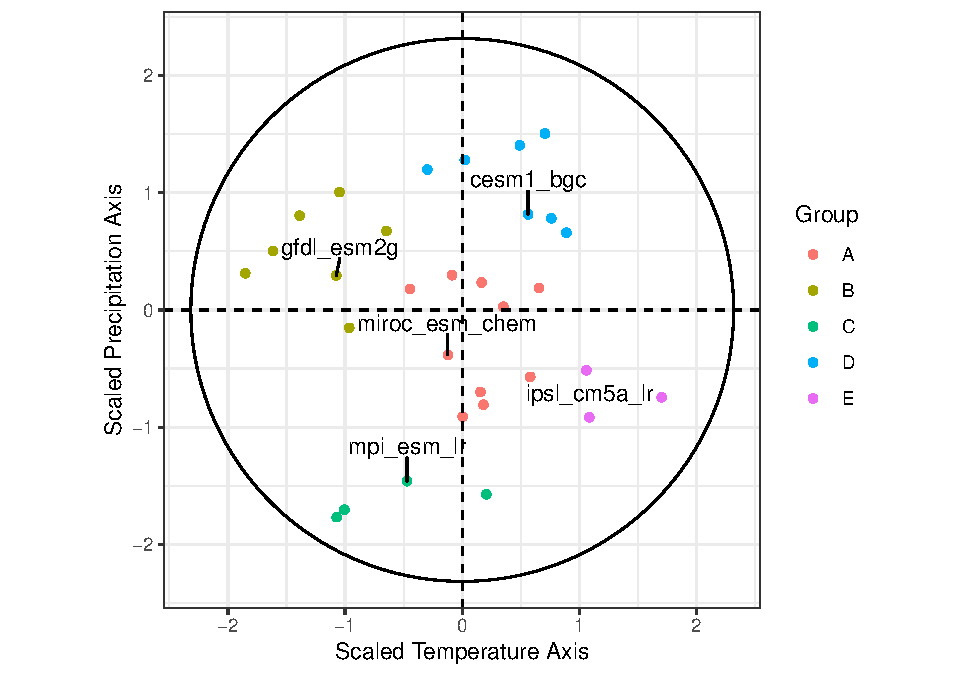
\includegraphics{Review_and_climate_files/figure-latex/SelectedGCMs-1.pdf}
\caption{\label{fig:SelectedGCMs}In this graph we can see the scaled temperature and precipitation axis, the center of the graph represent the ensemble of all models, the five groups represent the clusters selected using kmeans for five groups, the selected GCM of each cluster is shown with a label}
\end{figure}

\hypertarget{present-climate-conditions}{%
\subsubsection{Present climate conditions}\label{present-climate-conditions}}

Once the future GCM models were selected, the 30 seconds resolution maps were downloaded for 2070 and for present conditions from CHELSA \citep{karger2020high}.
The present conditions for the Los Lagos and Los Ríos Region are shown in Figure \ref{fig:PresenteClima}, with a close up to the 10 Km buffer surrounding the park in \ref{fig:PresenteClimaBuffer}. The region is a cold and humid area, with a range in the mean annual temperature from -5.6 to 13 degrees Celsius and a mean of 9.34, and a precipitation range between 858 to 4,537 and a mean of 2,092 mm a year.

\begin{figure}
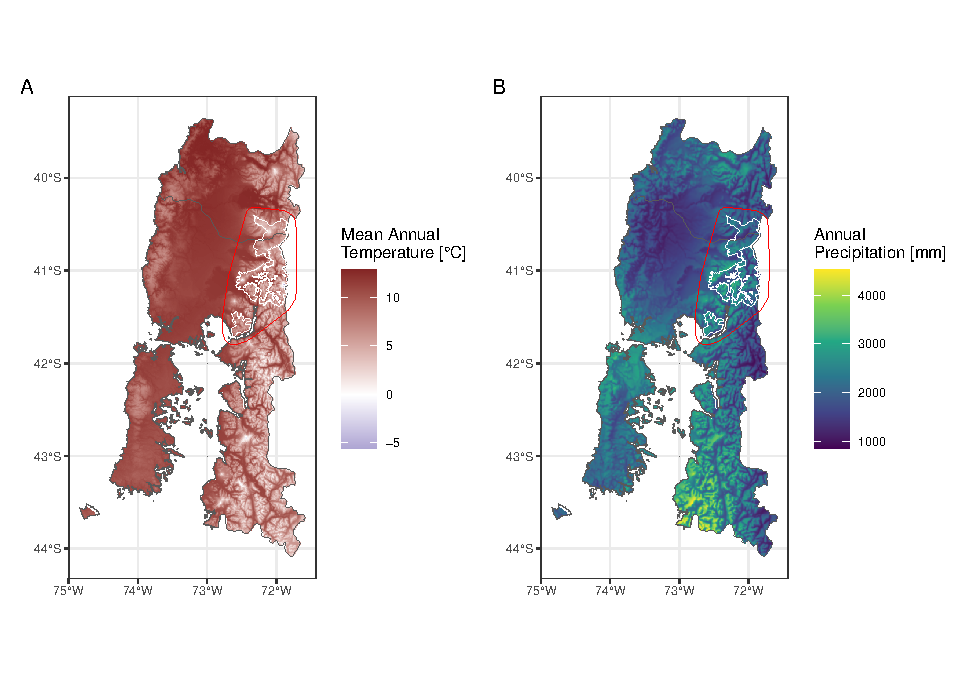
\includegraphics[width=1\linewidth,height=1\textheight]{Review_and_climate_files/figure-latex/PresenteClima-1} \caption{Mean anual temperature in °C (Facet A), and Annual Precipitation mm (Facet B)}\label{fig:PresenteClima}
\end{figure}

The parks considered in this project are in high altitude which leads to even cooler and wetter conditions, with a range from -5.6 to 12.6 and a mean of 8.12 degrees Celsius, and a precipitation range from from 1,176 to 3,410 and a mean of 2,134.51 mm as seen in figure \ref{fig:PresenteClimaBuffer}.

\begin{figure}
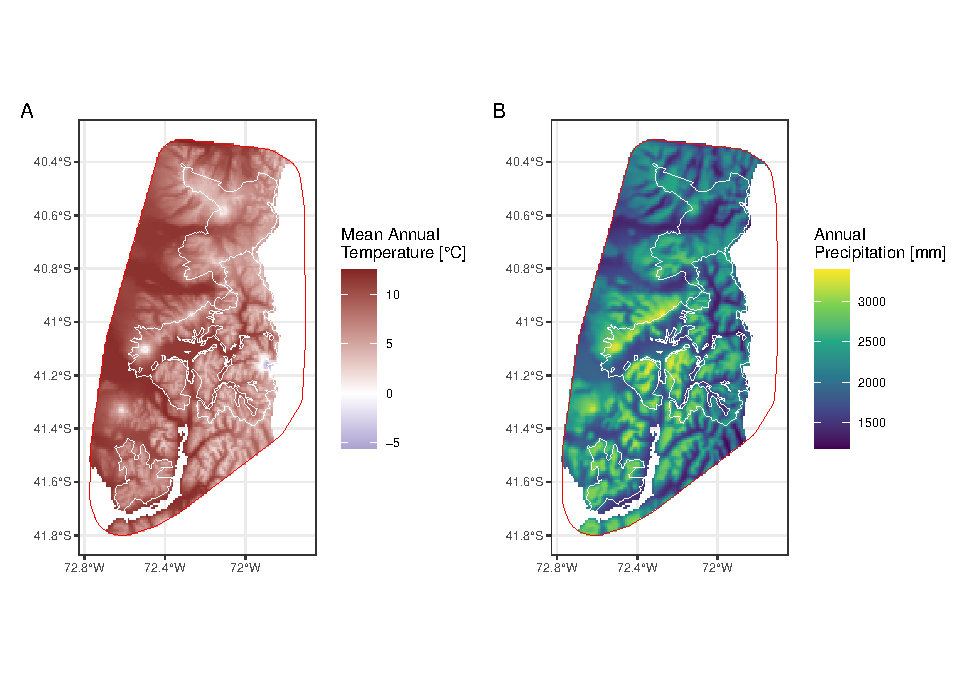
\includegraphics[width=1\linewidth,height=1\textheight]{Review_and_climate_files/figure-latex/PresenteClimaBuffer-1} \caption{Mean anual temperature in °C (Facet A), and Annual Precipitation mm (Facet B) in the three studied national parks white lines, and a 10 km buffer red line}\label{fig:PresenteClimaBuffer}
\end{figure}

\hypertarget{future-scenarios}{%
\subsection{Future scenarios}\label{future-scenarios}}

\hypertarget{future-temperature}{%
\subsubsection{Future temperature}\label{future-temperature}}

\begin{figure}
\centering
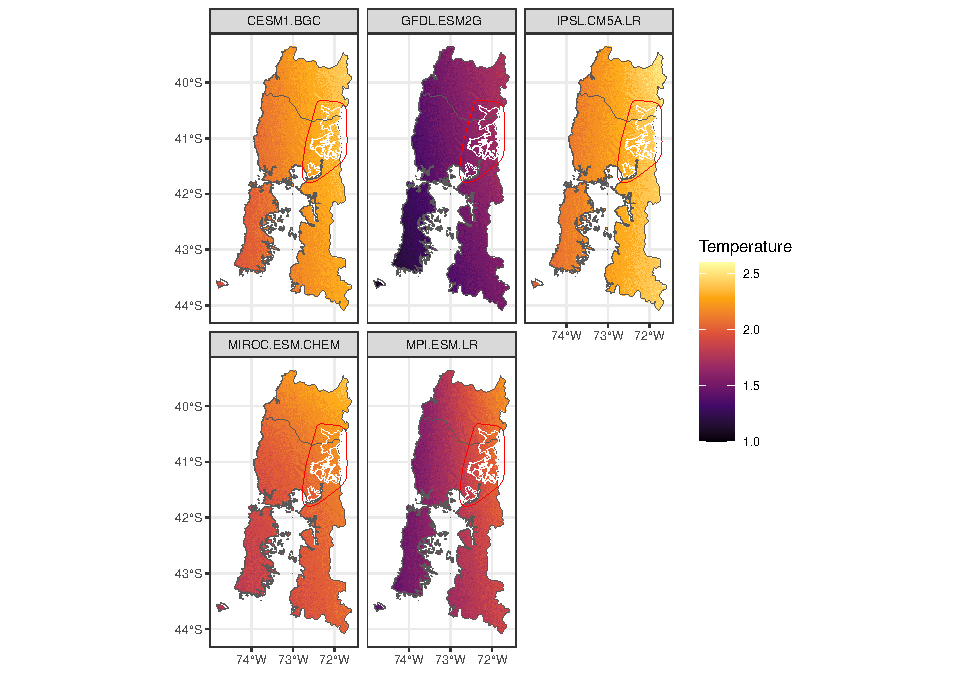
\includegraphics{Review_and_climate_files/figure-latex/DifTemp-1.pdf}
\caption{\label{fig:DifTemp}Changes in future mean annual temperature for the five selected GCMs, the red polygon surrounds the area of influence while the white line demarks the limits of the three protected areas in this proyect}
\end{figure}

As stated above, the four GCMs chosen to explore and model future scenarios are cesm1\_bgc, gfdl\_esm2g, ipsl\_cm5a\_lr, miroc\_esm\_chem and mpi\_esm\_lr. Even when this models include relatively wetter models such as cesm1\_bgc. On average for the whole region, the temperature will rise from 1.5 to 2.28 depending on the GCM (See figure \ref{fig:DifTemp}), but in some areas, it the temperature rise could be as high as 2.6 degrees Celsius.

As seen in figure \ref{fig:DifTempHull}, those changes are even higher within the parks and it's surrounding areas, which means the effects of climate change might be even greater.

\begin{figure}
\centering
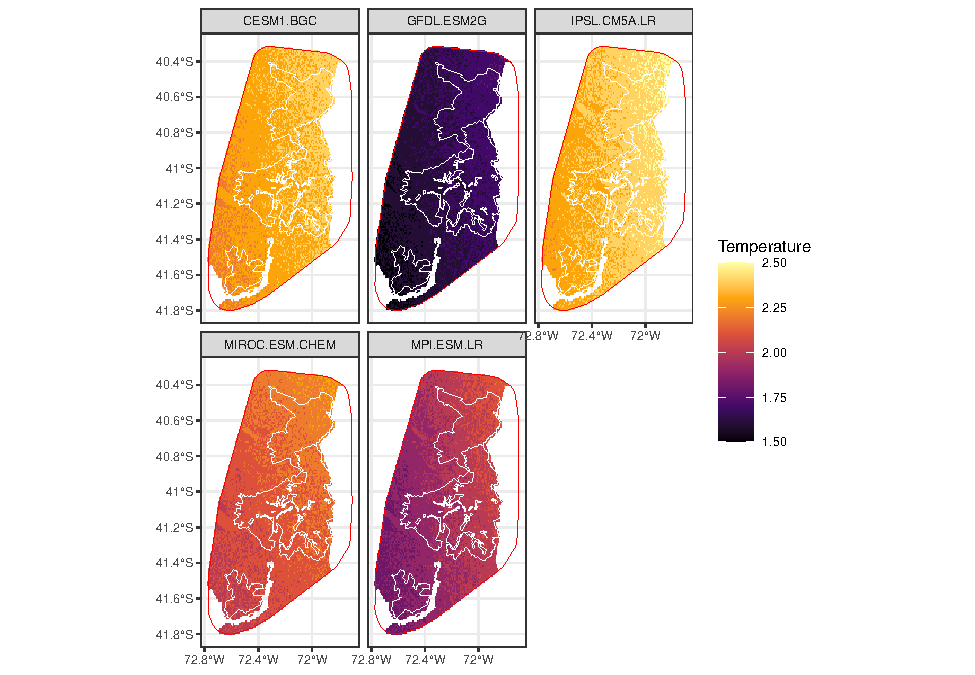
\includegraphics{Review_and_climate_files/figure-latex/DifTempHull-1.pdf}
\caption{\label{fig:DifTempHull}Temperature difference for all five GCMs, for the Close up of the area of influence of the parks}
\end{figure}

\hypertarget{future-precipitation}{%
\subsubsection{Future precipitation}\label{future-precipitation}}

The change in precipitation is predicted to be much more stark, with some areas decreasing in precipitation up to -696 as seen in figure \ref{fig:DifPrec}, this is particularly worrisome, since the ecosystems that are prevalent in the area depend on high precipitation.

\begin{figure}
\centering
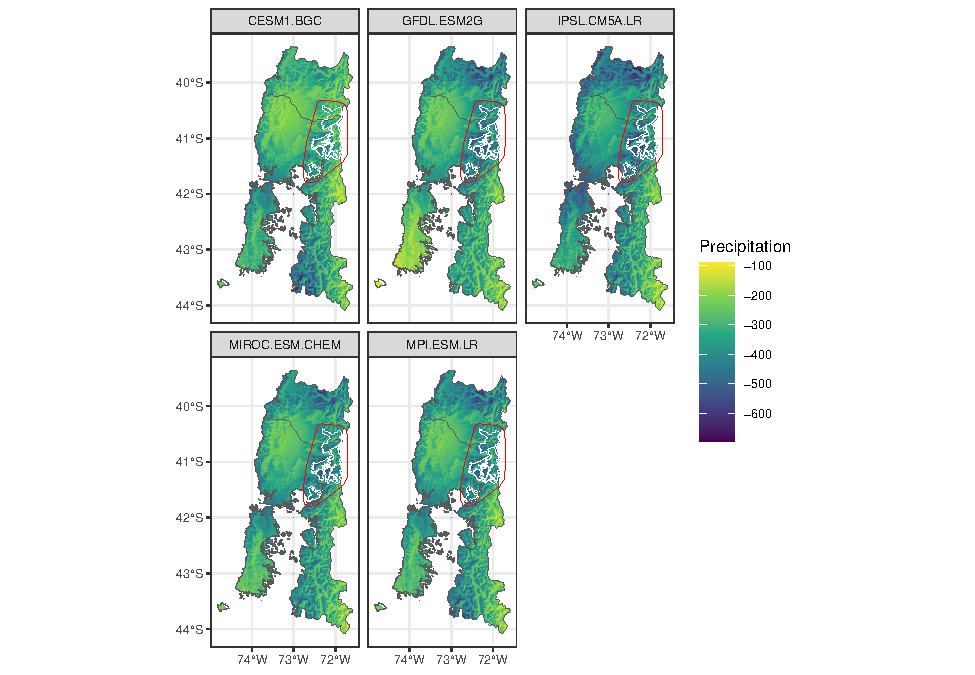
\includegraphics{Review_and_climate_files/figure-latex/DifPrec-1.pdf}
\caption{\label{fig:DifPrec}Changes in precipitation for the different GCMs, the red polygon surrounds the area of influence while the white line demarks the limits of the three protected areas in this proyect}
\end{figure}

\begin{figure}
\centering
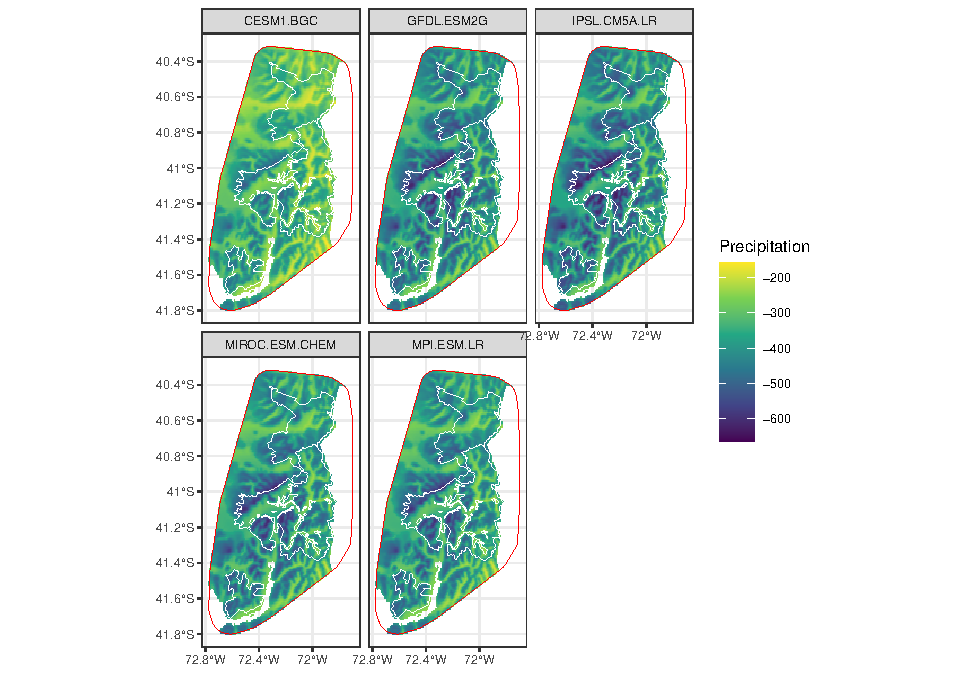
\includegraphics{Review_and_climate_files/figure-latex/DifPrecHull-1.pdf}
\caption{\label{fig:DifPrecHull}Precipitation difference for all five GCMs, for the Close up of the area of influence of the parks}
\end{figure}

The range of changes between GCMs will be from from -376.99 to -313.23 mean annual precipitation for the whole area. Again the areas where there is going to be a higher drop in precipitation are mostly inside of the national parks, as seen in figure \ref{fig:DifPrecHull}, with changes in the mean annual precipitation within the are of -412.29 for the wettest models, and -320.96 for the driest models.

\hypertarget{vegetation-formation}{%
\subsection{Vegetation formation}\label{vegetation-formation}}

We used \citet{luebert2009depuracion} to check current vegetation formations as seen in figure \ref{fig:VegHull}

\begin{figure}
\centering
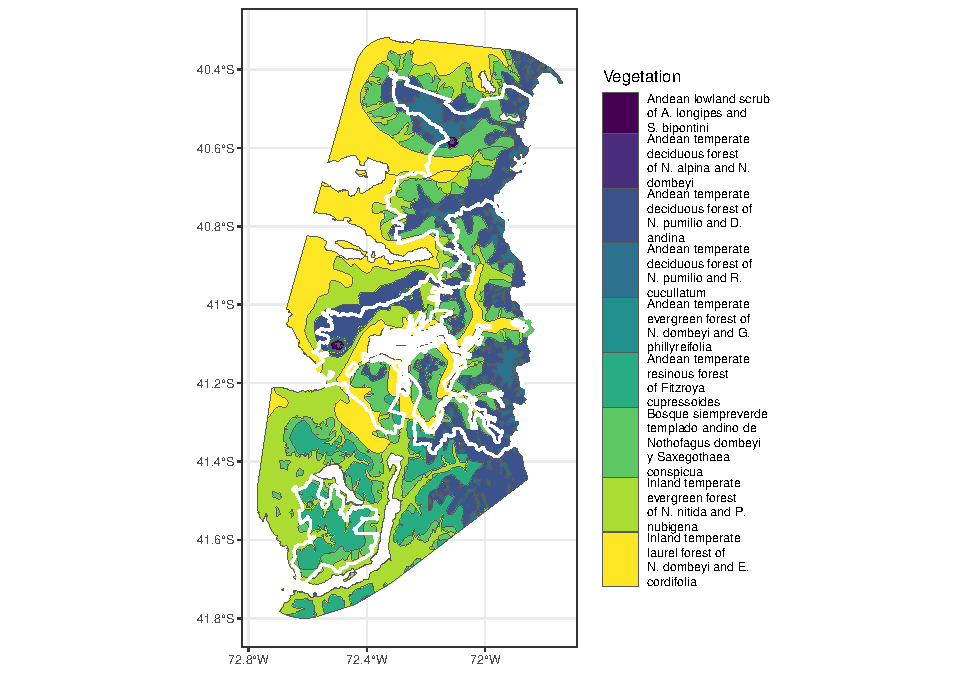
\includegraphics{Review_and_climate_files/figure-latex/VegHull-1.pdf}
\caption{\label{fig:VegHull}Vegetational formation in the influence area of the parks}
\end{figure}

\hypertarget{climatic-analogues}{%
\subsubsection{Climatic analogues}\label{climatic-analogues}}

As seen above, changes in precipitation will be very large. Because of that, we checked which areas in the present have the same climate as it is predicted to be in the future in the national parks and surrounding areas using the analogues R package \citep{ramirez2011climate}. After doing that, the current vegetation formations of those areas were checked in order to determine possible future vegetation in the area. With that we might better understand the biological consequences of climate change.

Currently in the National Parks and surrounding areas, the five most common Vegetation formations are Deciduous forest, Evergreen forest, Laurel forest, Low altitude scrubland and Resinous forest, and in the future, new vegetation formations that would be part of the five most common ones would include Absolute desert, Desert scrub, Sclerophyllous forest and Thorny forest. Of the current five most common formations, the ones that would be reduced as far as that they would either be lost completely or become very rare are Evergreen forest, Low altitude scrubland and Resinous forest

\begin{table}

\caption{\label{tab:TablaForm}Top five vegetation formations for the present and for the different GCMs according to the analogous climate analysis}
\centering
\fontsize{5}{7}\selectfont
\begin{tabular}[t]{lllllll}
\toprule
Rank & Present & CESM1-BGC & GFDL-ESM2G & IPSL-CM5A-LR & MIROC-ESM-CHEM & MPI-ESM-LR\\
\midrule
1 & Evergreen
forest & Deciduous
forest & Deciduous
forest & Deciduous
forest & Deciduous
forest & Deciduous
forest\\
2 & Deciduous
forest & Sclerophyllous
forest & Sclerophyllous
forest & Sclerophyllous
forest & Sclerophyllous
forest & Sclerophyllous
forest\\
3 & Laurel
forest & Desert
scrub & Thorny
forest & Desert
scrub & Desert
scrub & Desert
scrub\\
4 & Resinous
forest & Thorny
forest & Desert
scrub & Thorny
forest & Thorny
forest & Thorny
forest\\
5 & Low
altitude
scrubland & Laurel
forest & Laurel
forest & Absolute
desert & Laurel
forest & Laurel
forest\\
\bottomrule
\end{tabular}
\end{table}

\hypertarget{land-use}{%
\subsection{Land use}\label{land-use}}

We used \citet{zhao2016detailed} landuse layer, specifically developed for Chile. This is a 30 meter resolution, that

\includegraphics{Review_and_climate_files/figure-latex/unnamed-chunk-6-1.pdf}

\includegraphics{Review_and_climate_files/figure-latex/unnamed-chunk-7-1.pdf}

\begin{table}[H]
\centering
\begin{tabular}{lr}
\toprule
Primary landuse & Percentage\\
\midrule
forests & 59.17\\
grasslands & 12.95\\
Scrub & 10.24\\
Water bodies & 9.34\\
bare land & 6.93\\
\bottomrule
\end{tabular}
\end{table}

\begin{table}[H]
\centering
\begin{tabular}{lr}
\toprule
Secondary landuse & Percentage\\
\midrule
Native Broadleaf renoval & 39.45\\
Native Broad Leaf primary & 18.63\\
Scrub & 10.11\\
Lagos & 8.97\\
grasslands annual & 8.43\\
\addlinespace
Rocks rocky soils & 5.04\\
other Grasslands & 4.40\\
Rocky soil gravels & 1.85\\
\bottomrule
\end{tabular}
\end{table}

\renewcommand\refname{References}
\bibliography{Biblio.bib}

\end{document}
